\documentclass[10pt, landscape, a4paper]{article}
\usepackage{geometry}[landscape]
\usepackage{multicol}
\usepackage{graphicx}
\usepackage{amsmath} 
\usepackage{amssymb}
\usepackage{ccicons}
\usepackage{hyperref}

\usepackage[dvipsnames]{xcolor}

% Set page margins
\geometry{top=.8cm, left=.8cm, right=.8cm, bottom=.8cm}

% Set paragraph indentation
\setlength{\parindent}{0pt}

% Set path for assets
\graphicspath{{assets/}}

\setlength{\columnsep}{20pt}
\raggedcolumns

% _____ CUSTOM COMMANDS __________________________________________
\newcommand{\E}[0]{\mathbb{E}}
\newcommand{\R}[0]{\mathbb{R}}

\newcommand{\sgn}[0]{\text{sgn}}

\newcommand{\argmin}[1]{\underset{#1}{\text{argmin}}}
\newcommand{\argmax}[1]{\underset{#1}{\text{argmax}}}

\begin{document}
\begin{multicols*}{3}

% _____ CONTENT __________________________________________________

% main heading
\begin{center}
	\Large{\textbf{Visual Computing}} \\
    \small{by dcamenisch}
\end{center}

\section{Introduction}

This document is a summary of the 2022 edition of the lecture \textit{Visual Computing} at ETH Zurich. I do not guarantee correctness or completeness, nor is this document endorsed by the lecturers. If you spot any mistakes or find other improvements, feel free to open a pull request at \url{https://github.com/DannyCamenisch/vc-summary}. This work is published as CC BY-NC-SA.
\begin{center}
	\ccbyncsa
\end{center}
\section{The Digital Image}

An image is simply a continuous function over 2 or 3 variables (XY-coordinates and possibly time). Usually we use brightness as the value of the function, but other physical values can also be used. For a computer this is just a collection of numbers, but instead of continuous values we have discrete. Note that in real life images are never completely random and almost always contain some structure. It is important to know that \textbf{pixels are not little squares}, they are point measurements.

When taking a picture with a digital camera, we can encounter various problems, e.g.:
\begin{itemize}
	\item Transmission Interference
	\item Compression Artefacts
	\item Spilling
	\item Sensor Noise
\end{itemize}

\subsection{Sampling}

When taking an image, we are sampling such a continuous. When trying to reconstruct the original function, we can encounter undersampling, i.e. when we loose information due to a too low amount of sampling points. 

\begin{center}
	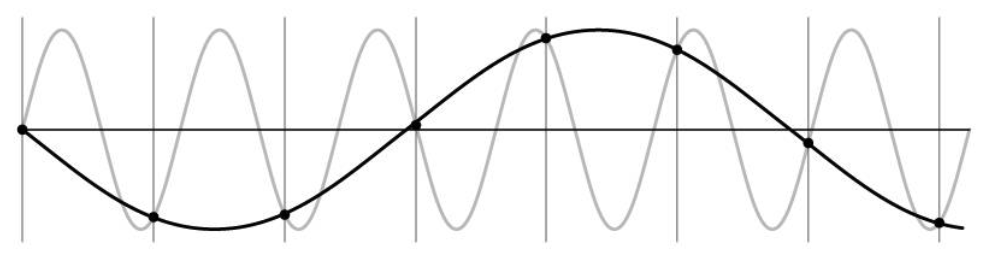
\includegraphics[width=0.8\linewidth]{undersampling.png}
\end{center}

Due to undersampling, the result can not be distinguished from a lower or a higher frequency wave. Signal disguised as other frequencies is also called \textbf{aliasing}. \medskip

\textbf{Nyquist-Shannon Sampling Theorem}

For sine waves we have to sample at half the wave length. This corresponds to double the frequency, we also call this the \textbf{Nyquist Frequency}.

\subsection{Quantization}

Another problem we have to deal with is \textbf{quantization}, since the real valued function will get digital (integer) values, it is lossy. Compared to sampling which lets us reconstruct the original function. Simple quantization uses equally spaced levels with $k$ intervals.

\begin{center}
	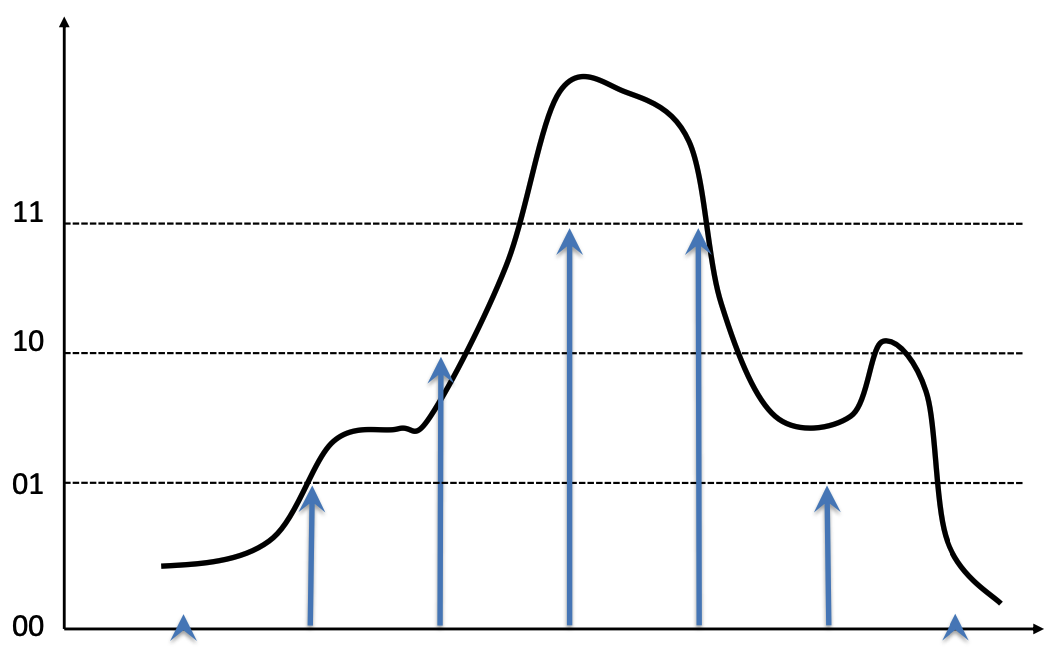
\includegraphics[width=0.8\linewidth]{quantization.png}
\end{center}

\subsection{Image Properties}

Image resolution is divided into two parts:
\begin{itemize}
	\item Geometric Resolution: How many pixels per area
	\item Radiometric Resolution: How many bits per pixel
\end{itemize}

\subsection{Noise}

When taking pictures we can almost always encounter some noise. A common way to model this is additive gaussian noise:
$$I(x,y) = f(x,y) + c, \qquad c \sim \mathcal N(0, \sigma^2)$$

The signal to noise ratio (SNR) is an index of image quality:
$$\text{SNR} = \frac{F}{\sigma}, \qquad F = \frac{1}{XY} \sum_{x=1}^{X}\sum_{y=1}^{Y} f(x,y)$$

The usefulness for this metric can vary drastically depending on the type of image (dark images will have a higher SNR compared to bright images). Therefore we introduce peak SNR:
$$\text{PSNR} = \frac{F_\text{max}}{\sigma}$$

\end{multicols*}
\end{document}

% ____ FOOTER ______________________________________________________
% Content and Template: 
% original by Danny Camenisch (dcamenisch@inf.ethz.ch), 2022
% based on different summaries from many helpful people